%% This is the impactor results chapter for my UBC PhD Dissertation
%% The parent document is called thesis.tex

\chapter{Impact and constant displacement rate loading change the surface strain and fractures of the femur in sideways fall simulation}
\label{ch:fracture}
Knowledge of proximal femur fracture initiation and progression could increase the ability predict who will suffer a hip fracture.
Initial failure locations could be important in the effort to increase the sensitivity of hip fracture screening techniques.
If failures start in one location, or in proximity to a certain type of structure, it may be possible to develop protocols that target these areas and identify if known morphologies that may lead to structural deficiency exist.
Additionally, knowledge of how the initial failure location influences the final fracture type may allow screening for those who could be susceptible to the most serious types of fractures.

Previous researchers have investigated failure locations~\citep{de_bakker_during_2009} and fracture patterns~\citep{backman_proximal_1957, lotz_use_1990, weber_proximal_1992, courtney_effects_1994, pinilla_impact_1996, keyak_prediction_2001, lochmuller_mechanical_2002, bell_structure_1999} in proximal femurs loaded to failure in materials testing machines.
These researchers used constant displacement rate loading techniques, some at low rates (\textless5~\ac{mm}/\ac{s}), and some at high rates (100~\ac{mm}/\ac{s}), to model a fall to the side.
While it has been shown that increasing displacement rate from 2 to 100~\ac{mm}/\ac{s} has only a modest effect on the ultimate strength of the proximal femur~\citep{courtney_effects_1994}, there are two questions that remain unanswered.
First, does 100~\ac{mm}/\ac{s} represent a real fall to the side, and secondly does the deformation of the bone, initial failure location or fracture type change when loading protocol is changed?

In Chapter~\ref{ch:behave_fail} I investigated the first of these issues, and this chapter concentrates on the questions of how the bone deforms and fails in the quasi-static, constant displacement rate and the impact fall simulations protocols.
Chapter~\ref{ch:behave_fail} investigated what loading protocol was appropriate for mechanical behaviour outcomes of the proximal femur, this chapter will inform researchers of the best protocol for investigating physical damage outcomes.
In this chapter, I investigate the strain developed on the surface of the proximal femur, as well as the changes in failure locations and final fracture types, with testing protocol as the independent variable.

Fracture of the proximal femur is preceded by the development of strain within the bone.
To assess the difference in the strain of the bone in the quasi-static, constant displacement rate apparatus and those loaded in the fall simulator, the surface strains on the anterior-superior neck of single specimens were compared between the two test conditions using \acf{dic}.

Comparison of the failure of the bones in the two tests conditions were done based on initial failure location, as well as final fracture pattern.
To compare these outcomes, two groups of similar specimens were loaded to failure, one using a quasi-static, constant displacement rate protocol, and the other using impact fall simulation.
The failure locations and fracture patterns were compared using categorical values and comparative diagrams.

A version of this chapter will be submitted to Osteoporosis International. 

\section{Introduction}
Hip fracture is a major orthopaedic burden, with reported averages of 20\% of orthopaedic beds being continuously occupied by hip fracture patients~\citep{lyritis_epidemiology_1992, borissova_femoral_2011}.
For this reason, researchers have striven to understand how fractures happen, and how those susceptible to fracture could be better identified.
Many experimental and computational tools have been developed to carry out this research, searching for clues that will enable clinicians to identify bones that are susceptible to fracture.

The experimental research has lead to correlations of fracture force with a number of different physical parameters including bone mineral density~\citep{boehm_prediction_2008, de_bakker_during_2009, lochmuller_mechanical_2002}, posture~\citep{pinilla_impact_1996, ford_effect_1996}, and displacement rates~\citep{courtney_effects_1994, weber_proximal_1992, gilchrist_mechanics_2013}.
Researchers who have investigated the influence of displacement rate on the failure load of the proximal femur saw a large increase in stiffness when the rate was changed from 2~to 100~\ac{mm}/\ac{s}, but only a small change in failure load~\citep{courtney_effects_1994}.
The small change in fracture load may be interpreted as a low dependence of failure mode on displacement rate, but failure is characterized by more than fracture load and the changes in other aspects of the failure, such as location, have never been experimentally investigated.

\sloppy
Bone is known to be viscoelastic~\citep{carter_compressive_1977, mcelhaney_dynamic_1966, crowninshield_response_1974, linde_mechanical_1991} and exhibit rate-dependent failure modes~\citep{mcelhaney_dynamic_1966, crowninshield_response_1974, carter_compressive_1977}.
Previous research into the dependence of proximal femur failure on displacement rate showed that increasing rates increased the ultimate strength of the bone in a dose dependent manner~\citep{courtney_effects_1994, weber_proximal_1992}.
No information was available on the locations of the initial fractures, but one study noted that the fracture type changed with displacement rate stating, ``there seemed to be a trend of trancervical fractures with slower loading and subtrochanteric fractures with faster loading"~\citep{weber_proximal_1992}.
\fussy

The dependence of strain development, initial fracture location and final fracture type on method of loading is yet unknown.
Previous work has demonstrated a large difference in mechanical behaviours (\ac{ie}, maximum force and energy to failure), but has not addressed changes in fracture locations or fracture types.
In this paper we aim to compare the strain fields in single specimens loaded using both quasi-static, constant displacement rate and fall simulation techniques.
We will compare \acf{dic} obtained maps of the minimum principal strain on the anterior-superior neck at the same compressive force in both techniques.
Additionally, fracture patterns and locations will be compared between two groups of specimens loaded to failure at constant displacement rate of 2~\ac{mm}/\ac{s}~\citep{nishiyama_proximal_2013}, or in a fall simulator designed to replicate the force-time response of the humna body during a fall to the side~\citep{gilchrist_development_2013}.
We hypothesized that
\begin{inparaenum}[(i)]
\item the strain fields observed on the femoral neck will be different;
\item the initial fracture locations will be different; and
\item the final fracture patterns will be different
\end{inparaenum}
between quasi-static, constant displacement rate and fall simulation testing.

\section{Materials and methods}
Twenty-four, fresh frozen human femora were acquired from consenting donors, in accordance with the ethics protocols of the University of British Columbia.
The donors had an average age of 77~(\ac{sd} = 10)~years and consisted of 19~females and 2~males.
Details of the 21 of the specimens that also had force-displacement data are available in a previously published companion paper~\cite{gilchrist_mechanics_2013}.
Three additional specimens were included for this analysis and their details are listed in Table~\ref{tab:additional_specimens}.
The specimens were cleaned of soft tissue and periosteum and a white-dot on black-background speckle pattern was applied to the anterior superior neck using an airbrush (VL, Paasche, Chicago, IL).
The black background was chosen to minimize glare and improve the \ac{dic} data quality.
The specimens were imaged using a clinical \ac{dxa} scanner (QRD 4500W, Hologic, Bedford, MA), with 4~\ac{kg} rice to simulate soft tissue~\cite{sran_accuracy_2004} to determine \ac{abmd} and osteoporosis classification.
This group of specimens will be referred to as the \textit{fall} group because they were fractured in the fall simulator.
The fall group specimens were loaded in two ways.
First, they were loaded to 50\% of their total \ac{abmd} predicted failure load~\cite{boehm_prediction_2008} in a materials testing machine, at a constant displacement rate of 0.5~\ac{mm}/\ac{s}.
These test results will be referred to as the fall:QS results, due to the quasi-static nature of the loading.
Following this, the fall specimens were loaded to failure in a fall simulator.
The results of the latter test will be referred to as the fall:FS results, due to the use of the fall simulator.

\begin{table}
\renewcommand{\arraystretch}{1.5}
\caption[Additional study specimens]{Donor information for additional specimens included in this study that are not included in~\citep{gilchrist_mechanics_2013}.}
\label{tab:additional_specimens}
\begin{tabular}{|c|c|c|c|c|c|}
\hline
Specimen & Side & Age & Gender & Total aBMD (g/cm\textsuperscript{2}) & \acs{op} Status \\
\hline
\hline
22 & R & 73 & F & 0.872 & Normal \\ \hline
23 & L & 72 & F & 0.964 & Normal \\ \hline
24 & L & 85 & F & \acs{na} & \acs{na} \\
\hline
\end{tabular}
\end{table}

In addition to the fall group, 20~fresh frozen human femora were loaded to failure at a constant displacement rate of 2~\ac{mm}/\ac{s} in a materials testing machine~\cite{nishiyama_proximal_2013}.
These specimens consisted of 20~femurs from 15~female and 5~male donors, with an average age of 77~(\ac{sd} = 13)~years, and were acquired and handled in accordance with the University of Calgary's ethics protocols.
This group of specimens will be called the \textit{slow} group because they were failed using a slow, constant displacement rate.
Soft tissue and periosteum were removed and \ac{dxa} scans were acquired using a clinical scanner (QDR4500, Hologic, Bedford, MA) to determine \ac{abmd} and osteoporosis state.
Further details of this specimen population are available in their original publication~\cite{nishiyama_proximal_2013}.

All specimens from both groups were potted in \acl{pmma}~(\acs{pmma}, Bosworth Co, Skokie, IL), in the literature-standard sideways fall orientation of 10$^\circ$ adduction and 15$^\circ$ internal rotation~\cite{courtney_effects_1994,pinilla_impact_1996,lochmuller_mechanical_2002,de_bakker_during_2009,manske_cortical_2008,manske_femoral_2006}, with 290--305~\ac{mm} from the distal pivot point to the most proximal point on the femoral head.
\ac{pmma} caps consisting of 20~\ac{g} of material formed into 3.5~\ac{cm} diameter disks, were moulded to the medial head and lateral trochanter with parallel surfaces to ensure even load application and prevent non-clinical isolated compression failures of the femoral head and lateral trochanter.

The bones in the fall group were loaded in two successive tests.
First, a materials testing machine (8874, Instron, Noorwood, MA) applied a sub-failure, quasi-static load at a constant displacement rate.
A preloaded of 100~\ac{n} was applied over 5~\ac{s} and held for 0.5~\ac{s} before loading the specimens to 50\% of their total aBMD predicted failure load~\cite{boehm_prediction_2008} at 0.5~\ac{mm}/\ac{s}.
Two high-speed video cameras (Phantom V12.1, Vision Research, Wayne, NJ) imaging at 100~\acf{fps}, and 1280x800~\ac{px} (17~\ac{px}/\ac{mm}), observed the anterior-superior femoral neck for \ac{dic}.
Following this test, the specimens were imaged using the planar X-ray to confirm no damage and transferred into the inertial fall simulator.

The fall simulator consisted of masses and springs selected to mimic the response of the body in a fall to the side.
The details of its design have described in detail elsewhere \cite{gilchrist_development_2013}, but briefly, it simulated the loading in a fall to the side using an lumped parameter model consisting of a body mass (32~\ac{kg}), a spring to replicate the pelvis (50~\ac{n}/\ac{mm}), mass to replicate the lateral pelvis and proximal femur (1.98~\ac{kg}), and closed cell foam to replicate the soft tissue over the trochanter (19~\ac{mm}).
The simulated fall was recorded by four high speed video cameras.
Two cameras observed the anterior-superior femoral neck at 10,000~\ac{fps} (Phantom V12.1), and a resolution of 1024x800~\ac{px} (15~\ac{px}/\ac{mm}) for \ac{dic} measurement.
One camera (Phantom V9) recorded the impact hammer and lateral trochanter at 9,216~\ac{fps} and 576x288~\ac{px} (5~\ac{px}/\ac{mm}) for trochanter displacement measurement, and lastly, one camera (Phatom V9) qualitatively observed the posterior of the specimen at 6,006~\ac{fps} and 480x480~\ac{px} for fracture monitoring.

The specimens in the slow group were loaded in the same materials testing machine, at a constant displacement rate at the greater trochanter of 2~\ac{mm}/\ac{s}, until fracture.
The tests were observed using two high speed video cameras (Phantom V12.1), aimed at the anterior and superior aspects of the specimens, recording at 500~\ac{fps} and 1280x800~\ac{px}.
No \ac{dic} data were acquired for the slow group.

For each specimen in the fall group, the surface topologies and minimum principal strains were measured using commercially available \ac{dic} software (DaVis v8.3, LaVision, G\"{o}ttingen, Germany).
Each specimen in the fall group had two \ac{dic} data sets consisting of the topology and minimum principal strains on the surface of the bone in the fall:\ac{QS} and fall:\ac{fs} conditions.
For each specimen in the fall group, \ac{dic}-derived strains and surfaces from both tests were extracted at the maximum force applied in the fall:\ac{QS} test.
An \ac{icp} algorithm was used to align the surface topologies, and strain data were then compared on a point-to-point basis.

Alignment of the surface topologies and analysis of the differences in strains were conducted using a custom \ac{cpp} algorithm (available in \S\ref{sec:code_dic_dic_register_compare}) utilizing the \ac{vtk} (5.10, Kitware, Clifton Park, NY).
Data were exported from DaVis, as two raster files, one with topology data, and the other with strain data.
The topology file contained (\textit{x, y}) data pairs and a \textit{z} height at each location.
The strain data file contained minimum principal strain at the same (\textit{x, y}) locations used in the topology file.
The two DaVis topology surfaces were read into memory and \ac{3d} meshes were created using Delaunay triangulation.
The strain files associated with each surface were then read in and the strain data were applied to each node in the triangulated mesh.
At this stage, two unaligned surfaces with strain data were contained in memory (Fig.~\ref{fig:OriginalPositions}).

\begin{figure}
\centering
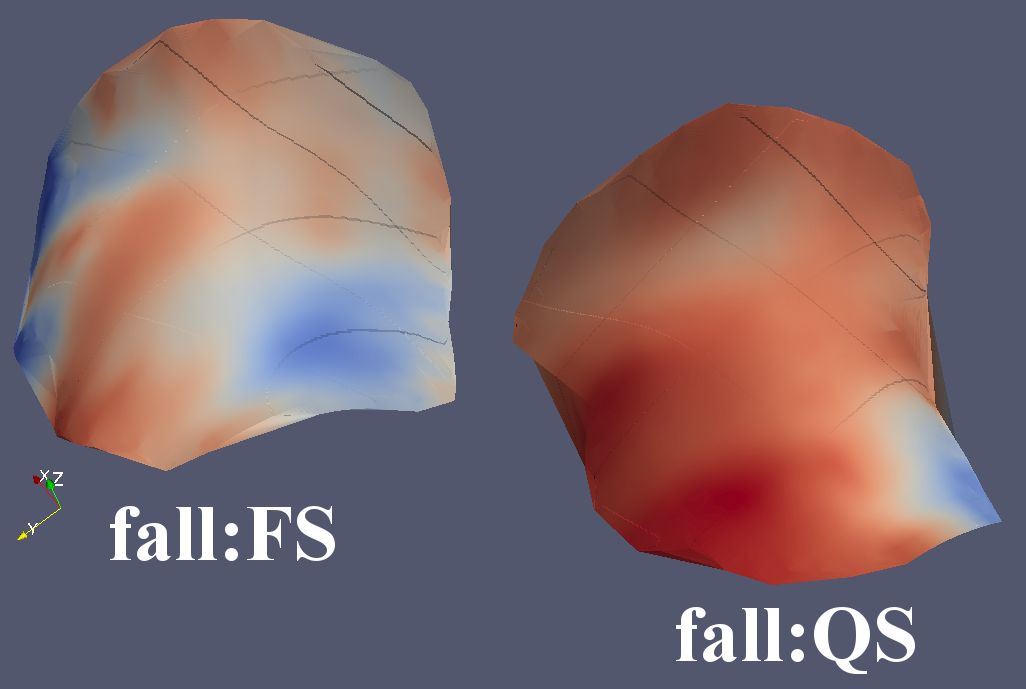
\includegraphics[width=0.7\linewidth]{./fracture/Figures/Original}
\caption[Original positions of the \acs*{dic} surfaces]{\textbf{The original positions of the surfaces from the quasi-static and fall simulation tests, coloured by minimum principal strain.} Image \copyright Seth Gilchrist, 2013}
\label{fig:OriginalPositions}
\end{figure}

Because the radius of convergence for \ac{icp} algorithms is small, a manual pre-alignment was required.
The pre-alignment was performed in ParaView (3.98.1, Kitware, Clifton Park, New York) and consisted three translations and three Euler angle rotations, which were passed to the \ac{icp} alignment program at runtime.

\begin{figure}
\centering
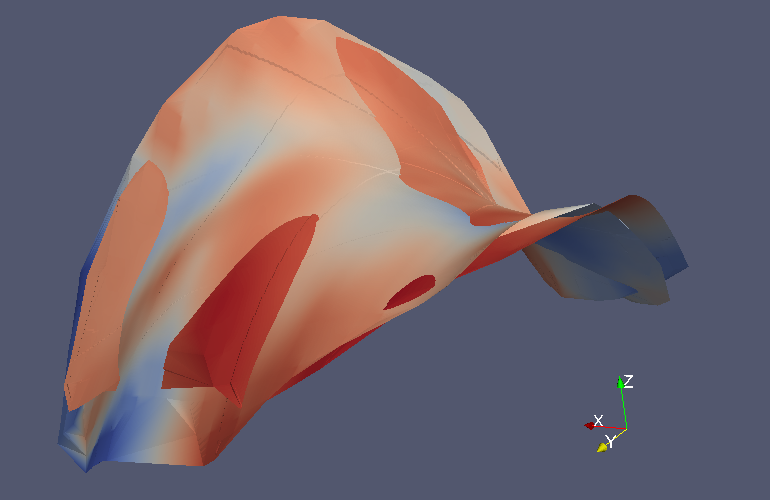
\includegraphics[width=0.7\linewidth]{./fracture/Figures/Aligned}
\caption[\acs*{dic} surfaces aligned after \acs*{icp}]{\textbf{\acs{dic} surface profiles after alignment using the \acs{icp} method.} Image \copyright Seth Gilchrist, 2013.}
\label{fig:AlignedPositions}
\end{figure}

While the profiles of the two surfaces were close, they did not match exactly, meaning that the data from one could not be readily compared to the other after the registration registration (Fig.~\ref{fig:AlignedPositions}).
To overcome this issue, an extrusion method was used to transfer data from the \ac{icp} target surface (the one that was stationary throughout registration) to the transformed surface.
Since the target surface was stationary throughout the registration, it was still aligned such that there were no occluded sections when viewed along the negative \textit{z}-direction.
Taking advantage of this, the target surface was extruded in the \textit{z}-direction to create a volume that enveloped the transformed surface (Fig.~\ref{fig:InstronExtruded}).
Once the extrusion had been performed, a copy was made of the transformed surface (including the strain data).
This copy was then trimmed using the bounds of the extruded target surface volume, creating a third surface (the \textit{master} surface) that consisted of only the overlapping regions of the two original surfaces (Fig.~\ref{fig:TransferData}).

\begin{figure}
\centering
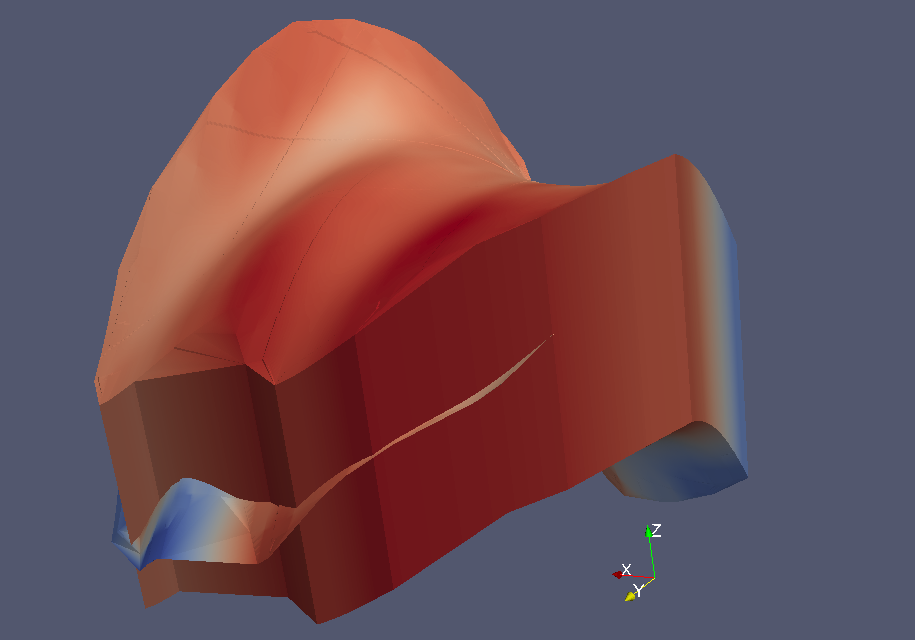
\includegraphics[width=0.7\linewidth]{./fracture/Figures/InstronExtruded}
\caption[\acs*{icp} target surface extruded]{\textbf{The \ac{icp} target surface was extruded in the z-direction, carrying all data with it. This ensured overlap with the transformed surface for data transfer.} Image \copyright Seth Gilchrist, 2013.}
\label{fig:InstronExtruded}
\end{figure}

\begin{figure}
\centering
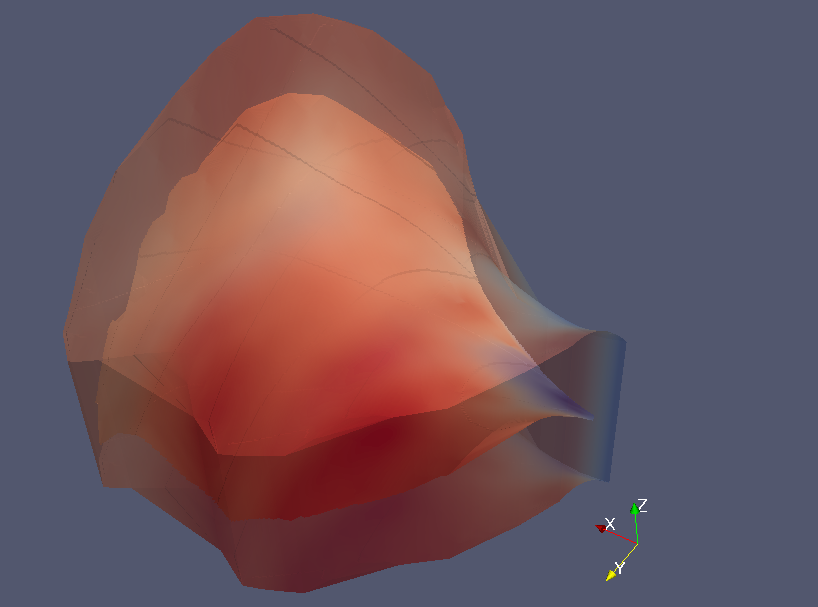
\includegraphics[width=0.7\linewidth]{./fracture/Figures/Transfer}
\caption[Transfer of \acs*{dic} data between surfaces]{\textbf{A trimmed version of the transformed surface was used as a master surface to compile all of the strain data from both the target and transformed surface in the region of overlap.} Image \copyright Seth Gilchrist, 2013.}
\label{fig:TransferData}
\end{figure}

After creating the master surface, the nodes of the master surface were used to probe the strain data in the extruded volume.
The strains were then stored in a new, point-associated dataset on the master surface.
At this stage, the master surface consisted only the overlapping regions of the original surfaces and contained all of the strain data from the original surfaces.
Calculations and statistics were performed on a point-by-point basis on the master surface (Fig.~\ref{fig:DuplicateSurfaceswithdata}).

\begin{figure}
\centering
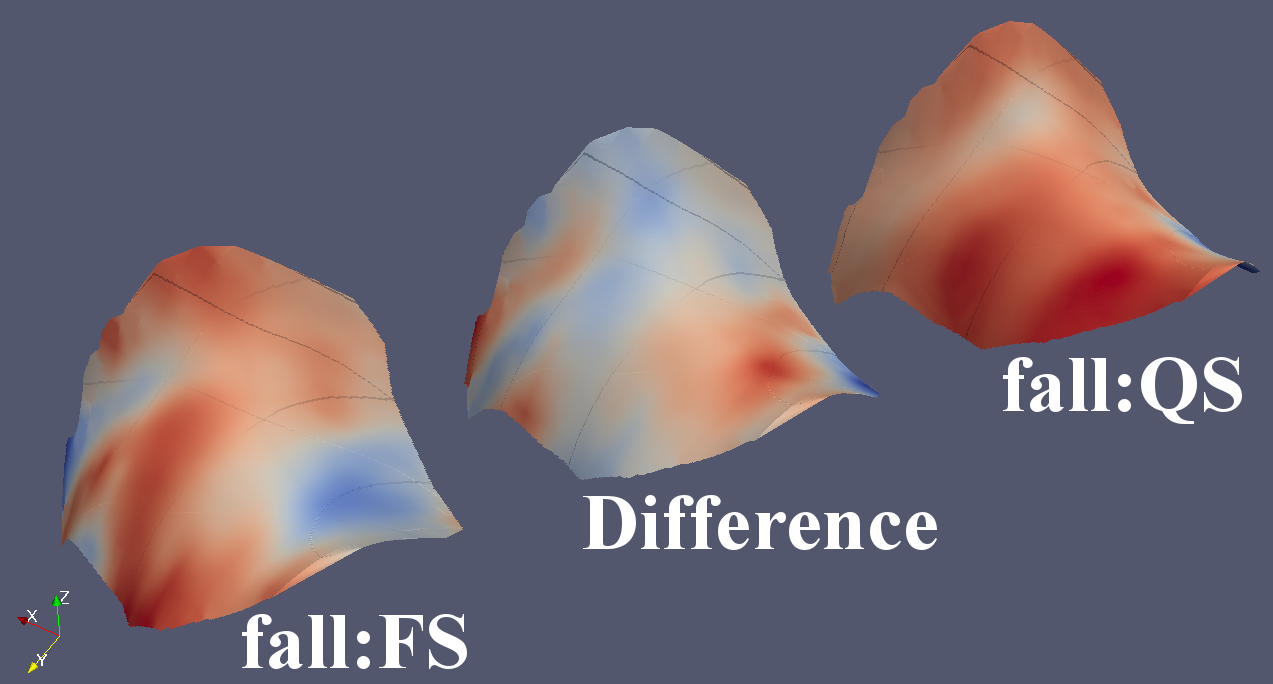
\includegraphics[width=0.7\linewidth]{./fracture/Figures/DuplicateSurfaceswithdata}
\caption[Surfaces to compare \acs*{dic} results]{\textbf{The fall simulator, quasi-static and master surfaces. In this image the master surface is showing the difference in strain between the fall:\ac{fs} and fall:\ac{QS} surfaces.} Image \copyright Seth Gilchrist, 2013.}
\label{fig:DuplicateSurfaceswithdata}
\end{figure}

The fall:\ac{fs} and slow group videos were reviewed to identify initial failure location, which was defined as the first location where yielding or crack formation was observed.
Initial failure locations were classified as one of,
\begin{inparaenum}[(a)]
\item superior neck,
\item inferior neck,
\item intertrochanteric,
\item trochanteric, or
\item no failure.
\end{inparaenum}
If the failure location could not be seen in the video, the specimen was not included in the statistical analysis for initial failure location.

Fracture was differentiated from failure in the analysis.
Fracture and was characterized by the loss of ability to withstand load and formation of fracture lines, whereas failure was characterized as formation of visible surface cracks, even when load was still supported.
Classifications were done by reconstructing the fragments and observations of the high speed video and were carried out by a fellowship-trained, orthopaedic trauma surgeon (author PG) and classified as,
\begin{inparaenum}[(a)]
\item \ac{neck},
\item \ac{is},
\item \ac{iu3},
\item \ac{iu4},
\item \ac{st}, or
\item \ac{nfx}.
\end{inparaenum}

The strain maps between the two loading conditions for the fall group were compared using match-pairs, Student's t-tests, where each point was considered to have two conditions, one for each loading scenario.
The fracture types and locations between the fall:\ac{fs} and slow group were compared using two-tailed Fisher Exact tests.
Additionally, initial failure locations were compared to final fracture lines to see if the initial location predicted the final fracture location.
Because the initial failure locations and fracture classifications were not comparable on a one-to-one basis, the analysis was simplified by grouping both classifications into either \textit{neck} or \textit{other} and placing the results into a 2x2 matrix with columns of initial locations and rows of final fracture location.
In the case were multiple fractures were observed, neck fractures were given precedent over trochanteric fractures, \ac{ie}, if both neck and trochanteric fractures were observed, the specimen was scored as a neck fracture.
A chi-squared test was used to determine if the initial failure location predicted the final fracture location.
Significance was set at $\alpha=0.05$ for all tests, and \textit{p}-values were adjusted for multiple comparisons using Holm's method.

\section{Results}
The fractures in the fall group showed significant variability (Fig.~\ref{fig:GilchristFractures}) and comminution, while the slow group (Fig.~\ref{fig:NishiyamaFractures}) showed relatively regular fracture lines, with little or no comminution.
In both tests crushing of the greater trochanter was seen under the \ac{pmma} pad.

Fracture types and initial location data (Tables~\ref{tab:GilchristFractures} and~\ref{tab:NishiyamaFractures}) showed that the two groups had significantly different fracture types ($p < 0.01$), but not significantly different initial failure locations ($p = 0.13$).
The fall:\ac{fs} group had more intertrochanteric fractures, which tended to be unstable.
Initial failure location predicted the final fracture location in the slow group ($p = 0.037$), but not in the fall:\ac{fs} group ($p=0.40$, Table~\ref{tab:initial_final_fast}).

The slow group specimens suffered fractures in all cases.
This is to be expected as the test protocol called for displacement of the greater trochanter well beyond the elastic range for the bones.
In the fall group, failure was seen in all cases but fracture was seen in only 22 of the 24 specimens.
In the two non-failure cases (specimens~3 and~19) cracks were observed in the video and post fracture analysis, but the specimens did not fracture, meaning that the bones retained load bearing capacity and had no open fractures.

\begin{figure}
	\centering
	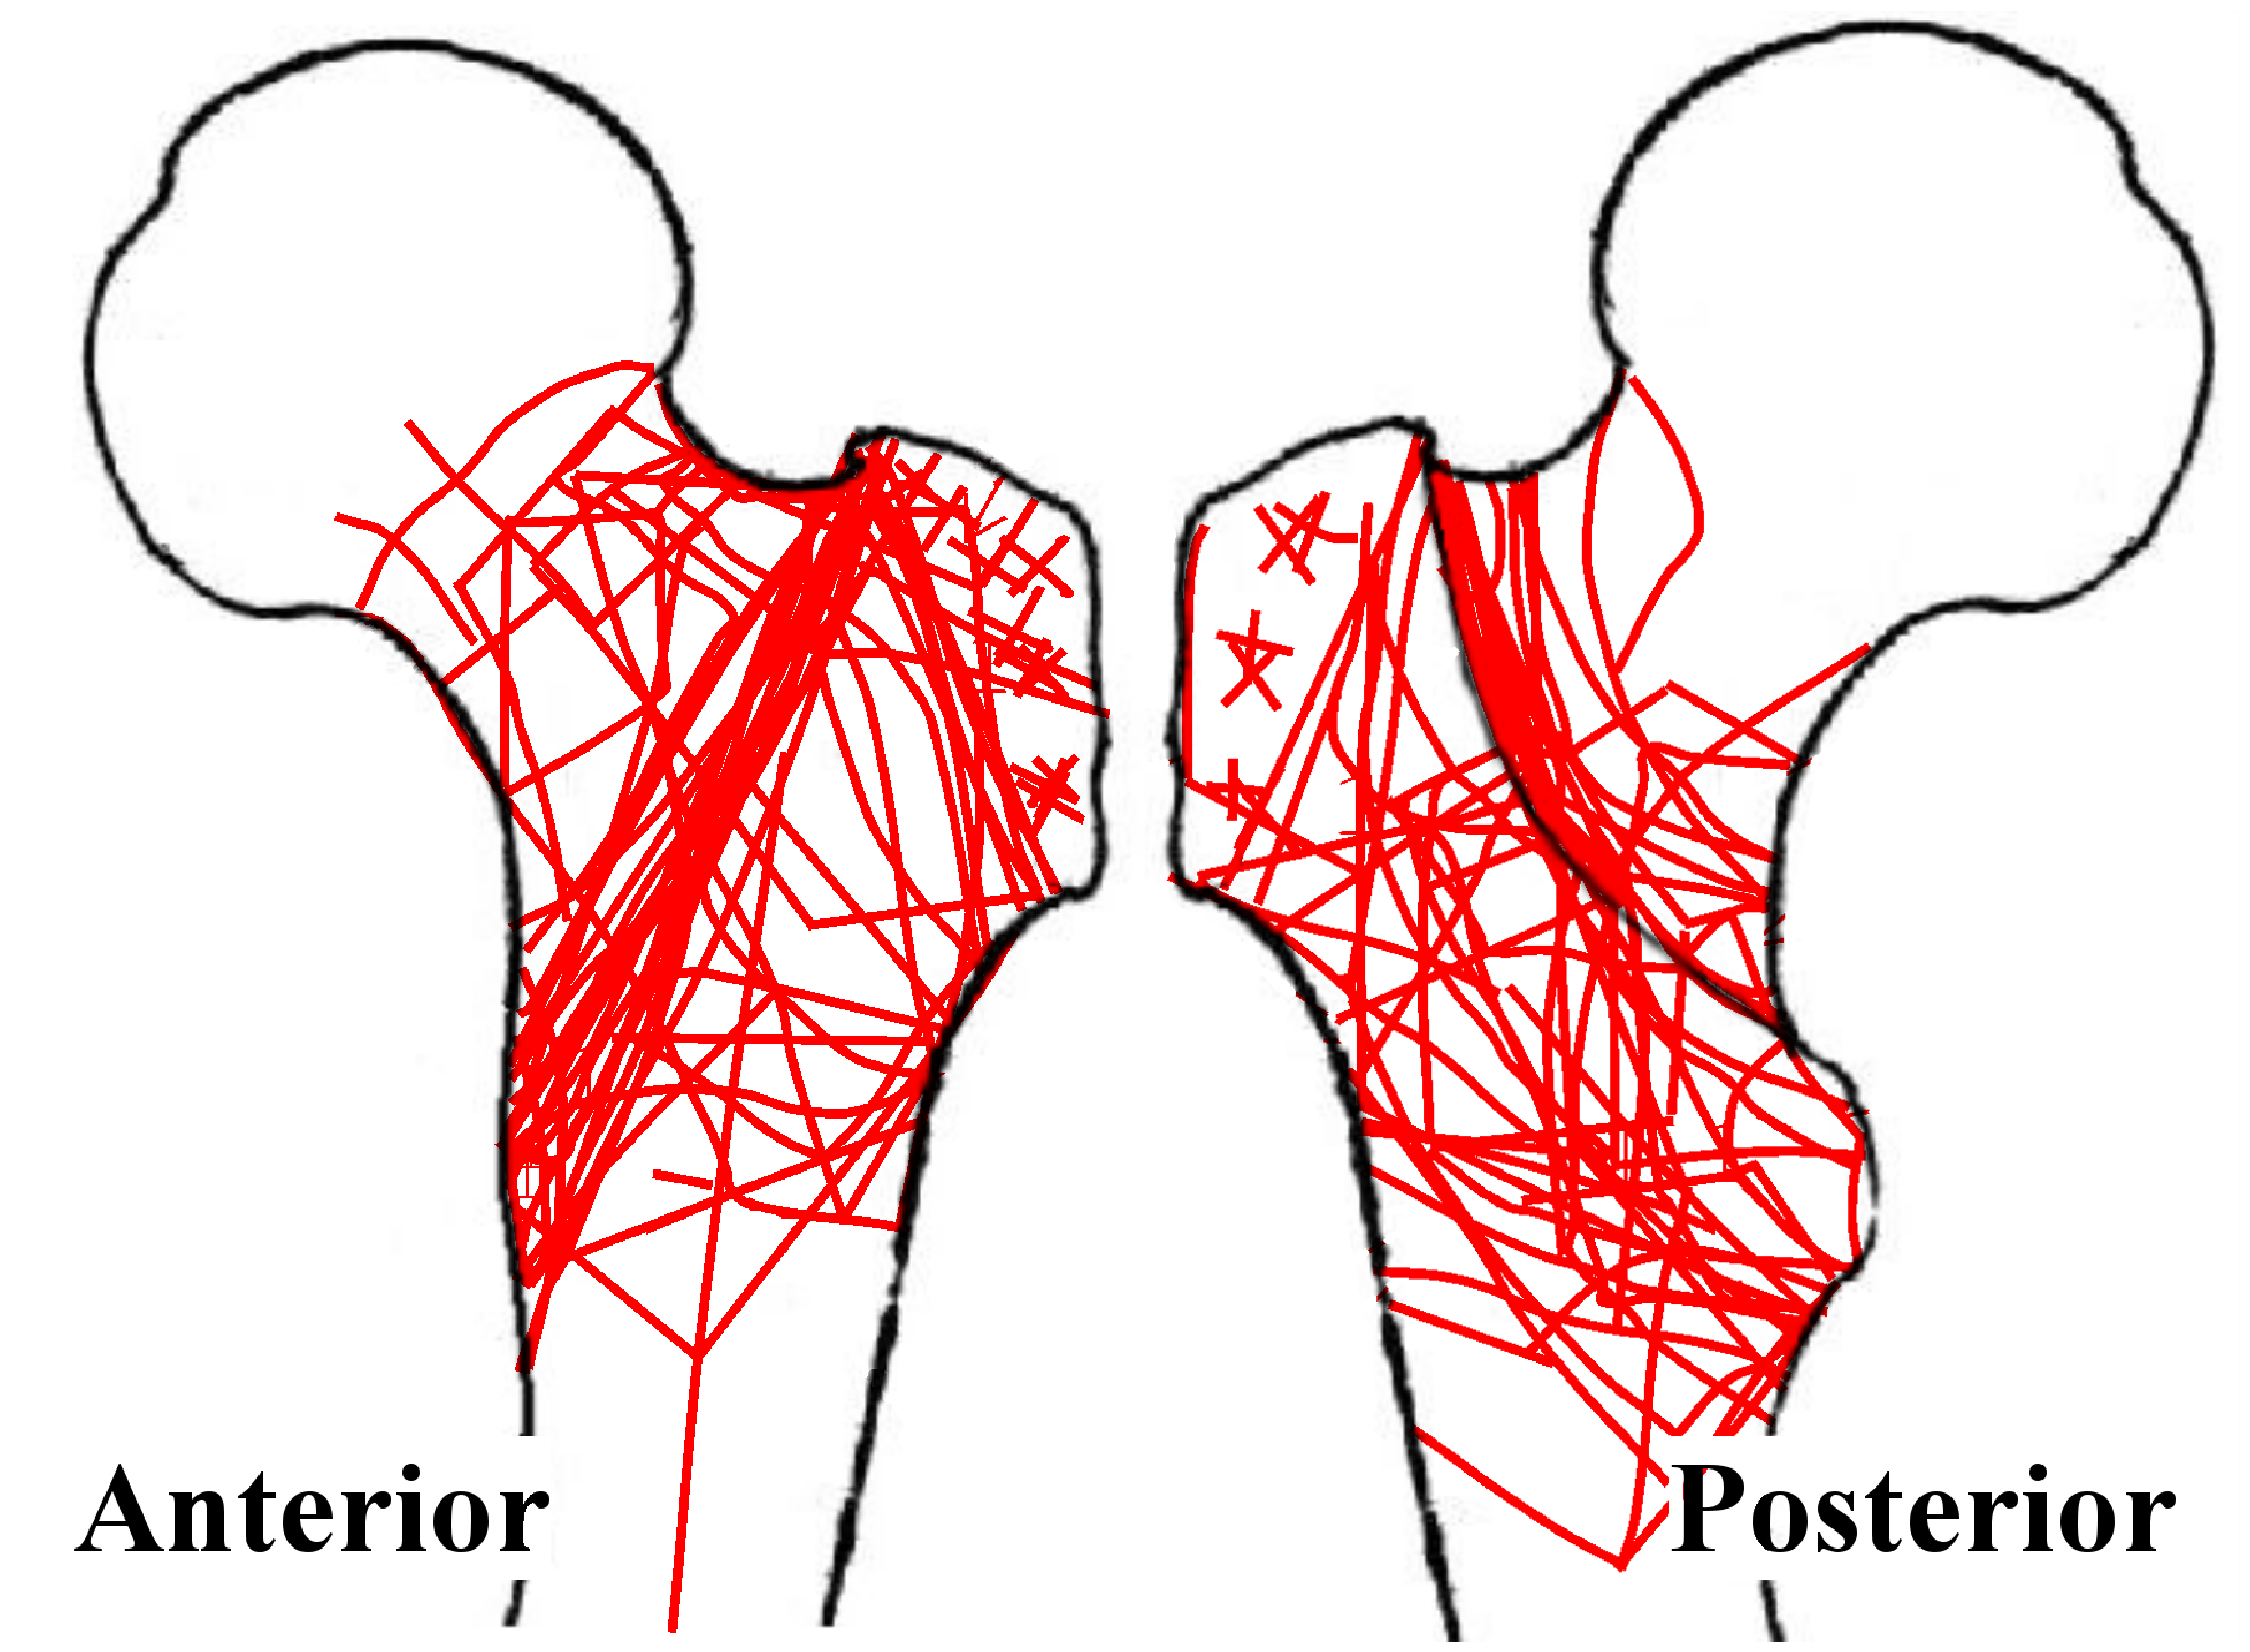
\includegraphics[width=0.7\linewidth]{./fracture/Figures/GilchristFractures.eps}
	\caption[Fall:\acs*{fs} group fracture lines]{\textbf{Fracture lines observed in the fall:\ac{fs} group compiled onto a single femur profile.} Graphic \textcopyright Seth Gilchrist, 2013.}
	\label{fig:GilchristFractures}
\end{figure}

\begin{table}
	\begin{center}
		\caption[Failure locations and fracture types for simulated group]{Initial failure locations and final fracture types for the specimens in the fall:\ac{fs} group} % N = neck, IS = intertrochanteric stable, IU3 = intertrochanteric unstable 3-part, IU4 = intertrochanteric unstable 4-part, ST = subtrochanteric, NFx = no fracture.}
		\label{tab:GilchristFractures}
		\begin{tabular}{|c||>{\centering}p{2em}|>{\centering}p{2em}|>{\centering}p{2em}|>{\centering}p{2em}|>{\centering}p{2em}|>{\centering}p{2em}|c|}
			\hline 
			\multirow{2}{*}{Specimen}	& \multicolumn{6}{c|}{Fracture Types}	 & \multirow{2}{*}{\lbCell{Initial Failure \\ Location}} \\ \cline{2-7}
		 & \ac{neck} & \ac{is} & \ac{iu3} & \ac{iu4} & \ac{st} & \ac{nfx} & \\ \hline
			\hline 1 		& \checkmark &  & & \checkmark & & 	& Intertrochanteric \\
			
			\hline 2 		&  & \checkmark &  &  &  & 			& Intertrochanteric \\
			
			\hline 3 		&  &  &  &  &  & \checkmark			& Superior Neck		\\
			
			\hline 4 		& \checkmark &  & \checkmark &  & \checkmark & 	& Trochanteric 		\\ 
			
			\hline 5 		&  &  & \checkmark &  &  & 			& Intertrochanteric \\ 
			
			\hline 6 		& \checkmark &  & \checkmark &  &  &  	& Trochanteric		\\ 
			
			\hline 7 		&  &  & \checkmark &  &  & 			& Trochanteric		\\ 
			
			\hline 8 		& \checkmark &  &  &  &  & 			& Superior Neck		\\ 
			
			\hline 9 		&  &  &  & \checkmark &  & 			& Trochanteric		\\ 
			
			\hline 10 		& \checkmark &  &  & \checkmark &  & & Trochanteric		\\
			
			\hline 11 		& \checkmark &  &  &  &  &			& Superior Neck		\\ 
			
			\hline 12 		&  &  & \checkmark &  &  &  		& Trochanteric		\\ 
			
			\hline 13 		&  &  & \checkmark &  &  & 			& Intertrochanteric	\\ 
			
			\hline 14 		&  &  &  &  &  & \checkmark			& Trochanteric		\\ 
			
			\hline 15 		&  & \checkmark &  &  &  & 			& Intertrochanteric	\\ 
			
			\hline 16 		& \checkmark &  & \checkmark &  &  & & Intertrochanteric	\\ 
			
			\hline 17 		&  & \checkmark &  &  &  & 			& Intertrochanteric	\\ 
			
			\hline 18 		& \checkmark &  & \checkmark &  &  & & Intertrochanteric	\\ 
			
			\hline 19 		&  & \checkmark &  &  &  & 			& Trochanteric		\\ 
			
			\hline 20 		&  & \checkmark &  &  &  &  		& Intertrochanteric	\\ 
			
			\hline 21		&  &  & \checkmark &  &  &  		& Trochanteric		\\ 

			\hline 22 		& \checkmark &  &  &  & \checkmark & 			& Superior Neck 	\\ 
			
			\hline 23 		& \checkmark & \checkmark &  &  &  &  			& Trochanteric 		\\ 

			\hline 24 		& \checkmark &  &  &  &  &  		& Not Available		\\ 
			
			\hline 
		\end{tabular} 
	\end{center}
\end{table}

\begin{figure}
	\centering
	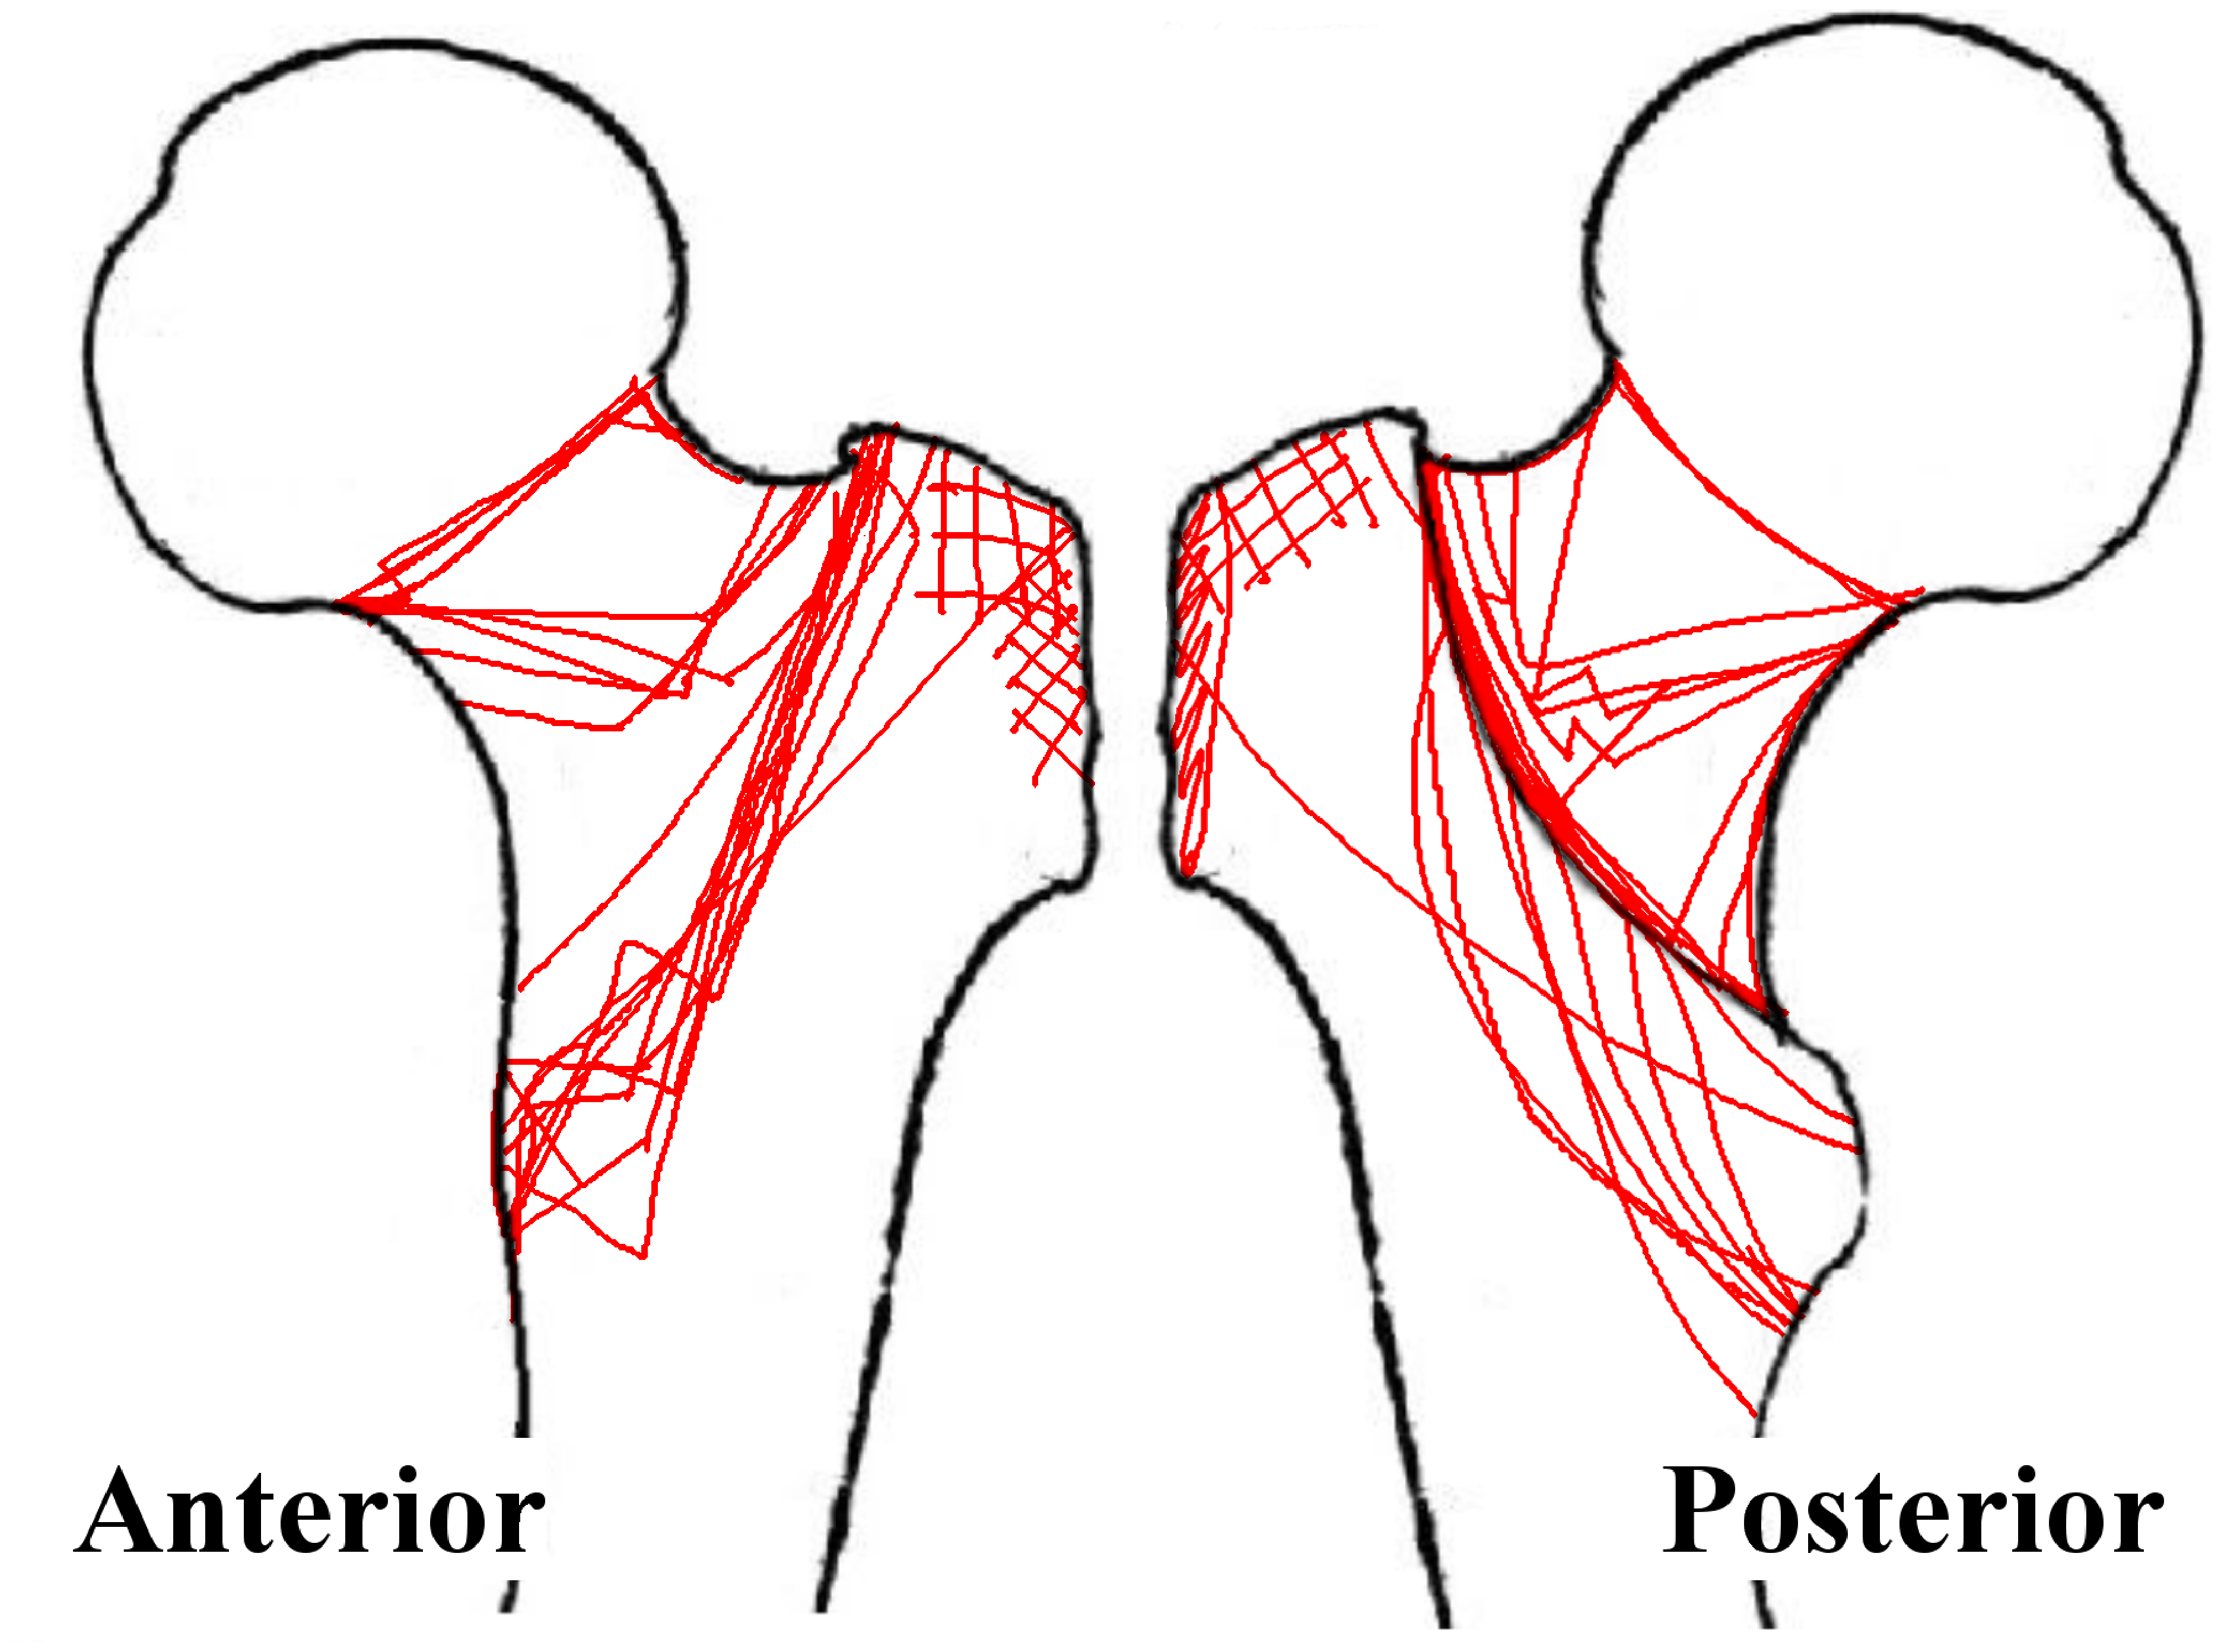
\includegraphics[width=0.7\linewidth]{./fracture/Figures/NishiyamaFractures.eps}
	\caption[Slow group fracture lines]{\textbf{Fracture lines observed in the slow group compiled onto a single femur profile.} Graphic \textcopyright Seth Gichrist, 2013.}
	\label{fig:NishiyamaFractures}
\end{figure}

\begin{table}
	\begin{center}
		\caption[Failure locations and fracture types for slow group]{Initial failure locations and final fracture types for the specimens slow group} % N = neck, IS = intertrochanteric stable, IU3 = intertrochanteric unstable 3-part, IU4 = intertrochanteric unstable 4-part, ST = subtrochanteric, NFx = no fracture. }
		\label{tab:NishiyamaFractures}
		\begin{tabular}{|c||>{\centering}p{2em}|>{\centering}p{2em}|>{\centering}p{2em}|>{\centering}p{2em}|>{\centering}p{2em}|>{\centering}p{2em}|c|}
			\hline 
			\multirow{2}{*}{Specimen}	& \multicolumn{6}{c|}{Fracture Types}	 & \multirow{2}{*}{\lbCell{Initial Failure \\ Location}} \\ \cline{2-7}
			 & \ac{neck} & \ac{is} & \ac{iu3} & \ac{iu4} & \ac{st} & \ac{nfx} & \\ \hline
			
			\hline 1		&  &  & \checkmark &  &  & 			& Intertrochanteric	\\ 
			
			\hline 2		&  &  & \checkmark &  & &			& Intertrochanteric	\\ 
			
			\hline 3		&  & \checkmark &  &  &  & 			& Intertrochanteric	\\ 
			
			\hline 4		& \checkmark &  &  &  &  &  		& Superior Neck		\\ 
			
			\hline 5		&  & \checkmark &  &  &  &  		& Unknown		\\ 
			
			\hline 6		&  & \checkmark &  &  &  &  		& Intertrochanteric	\\ 
			
			\hline 7		& \checkmark &  &  &  &  & 			& Superior Neck		\\ 
			
			\hline 8		& \checkmark &  &  &  &  & 			& Superior Neck		\\ 
			
			\hline 9		&  & \checkmark &  &  &  &  		& Intertrochanteric	\\ 
			
			\hline 10		& \checkmark &  &  &  &  & 			& Superior Neck		\\ 
			
			\hline 11		&  & \checkmark &  &  &  &  		& Unknown		\\ 
			
			\hline 12		& \checkmark &  &  &  &  & 			& Superior Neck		\\ 
			
			\hline 13		& \checkmark &  &  &  &  & 			& Intertrochanteric	\\ 
			
			\hline 14		& \checkmark &  &  &  &  & 			& Unknown		\\ 
			
			\hline 15		&  & \checkmark &  &  &  &  		& Intertrochanteric	\\ 
			
			\hline 16		& \checkmark &  &  &  &  & 			& Superior Neck		\\ 
			
			\hline 17		& \checkmark &  &  &  &  & 			& Inferior Neck		\\ 
			
			\hline 18		&  & \checkmark &  &  &  &  		& Unknown		\\ 
			
			\hline 19		&  & \checkmark &  &  &  &  		& Superior Neck		\\ 
			
			\hline 20		&  & \checkmark &  &  &  &  		& Intertrochanteric	\\ 
			
			\hline 
		\end{tabular}
	\end{center}
\end{table}

\begin{table}
\caption[Initial failure and final fracture locations]{Initial failure locations and final fracture locations in each group}
\label{tab:initial_final_fast}
\begin{subtable}{0.45\textwidth}
\centering
\caption{Fall:\ac{fs} group}
\begin{tabular}{r c c c}
 & & \multicolumn{2}{c}{Initial} \\
 & & \multicolumn{1}{|c|}{Neck} & \multicolumn{1}{c|}{Other} \\
 \cmidrule{2-4}
 \multirow{2}{*}{\rotatebox{90}{Final}} & \multicolumn{1}{c|}{Neck} & \multicolumn{1}{c|}{3} & \multicolumn{1}{c|}{7} \\
 \cmidrule{2-4}
  & \multicolumn{1}{c|}{Other} & \multicolumn{1}{c|}{1} & \multicolumn{1}{c|}{12}\\
 \cmidrule{2-4}
\end{tabular}
\end{subtable}
\begin{subtable}{0.45\textwidth}
\centering
\caption{Slow group}
\begin{tabular}{r c c c}
 & & \multicolumn{2}{c}{Initial} \\
 & & \multicolumn{1}{|c|}{Neck} & \multicolumn{1}{c|}{Other} \\
 \cmidrule{2-4}
 \multirow{2}{*}{\rotatebox{90}{Final}} & \multicolumn{1}{c|}{Neck} & \multicolumn{1}{c|}{7} & \multicolumn{1}{c|}{1} \\
 \cmidrule{2-4}
  & \multicolumn{1}{c|}{Other} & \multicolumn{1}{c|}{1} & \multicolumn{1}{c|}{7}\\
 \cmidrule{2-4}
\end{tabular}
\end{subtable}
\end{table}

The comparison of the surface strains in the fall:\ac{QS} and fall:\ac{fs} tests at the same load, and location showed that there were significant differences between the test conditions ($p < 0.01$, Fig.~\ref{fig:StrainDiffs}).
When all fall group data were pooled, the fall:\ac{QS} strain was 221~\ac{micro-eps} higher than the fall:\ac{fs} strain ($p = 0.45$, 95\%~\acs{ci}~=~(921,~-477)), which was 6.9\% of the average quasi-static strain of -3205~\ac{micro-eps}.

Comparison of the strain fields showed that they were typically correlated, but often exhibited an offset in the measured strain (Fig.~\ref{fig:StrainDiffs}).
The average \acs{rms} error in the surface matching was 5.3*10\textsuperscript{-11}~\ac{m}, indicating that the majority of the 50,000+ points in each surface were nearly coincident after the registration.
Some of the strain comparisons displayed ``branches" on the strain-strain plots (specimens 15, 24, 25 and 26), which were indicative of a redistribution of the strain field.
To illustrate this, specimen 24, which showed two branches in the strain-strain plot (Fig.~\ref{fig:StrainDiffs}), was seen to have two locations where the strains were different, one on the lateral neck and the other in the sub-capital region (Fig.~\ref{fig:H1380R_FemurOverlay}).
The locations of the differences in strain were qualitatively examined in specimens 15, 24, 25 and 26 and the redistributions did not seem systematic, rather they appeared random.

\section{Discussion}
This experiment studied the strain distributions, failure locations and fracture patterns between quasi-static, fixed displacement rate and impact fall simulation loading protocols.
The failure study showed that final fracture patterns were significantly different between the two groups, even though the initial failure locations were not.
This leads us to reject the null hypotheses that fracture types are the same between quasi-static and fall simulation testing, and accept the null hypothesis that initial failure locations are the same in both testing methods.
The strain between the two sub-failure tests conditions were significantly different on a point by point basis, but when pooled together there was no significant trend.
Therefore, testing of the hypothesis that there would be a significant difference in strain lead to two solutions, firstly, we reject the null hypothesis that there would be no difference in strain on any given proximal femur between the two testing methods, however, we accept the null hypothesis that there is no significant difference between the testing methods on a population level.

\afterpage{
\begin{landscape}
\begin{figure}
	\centering
	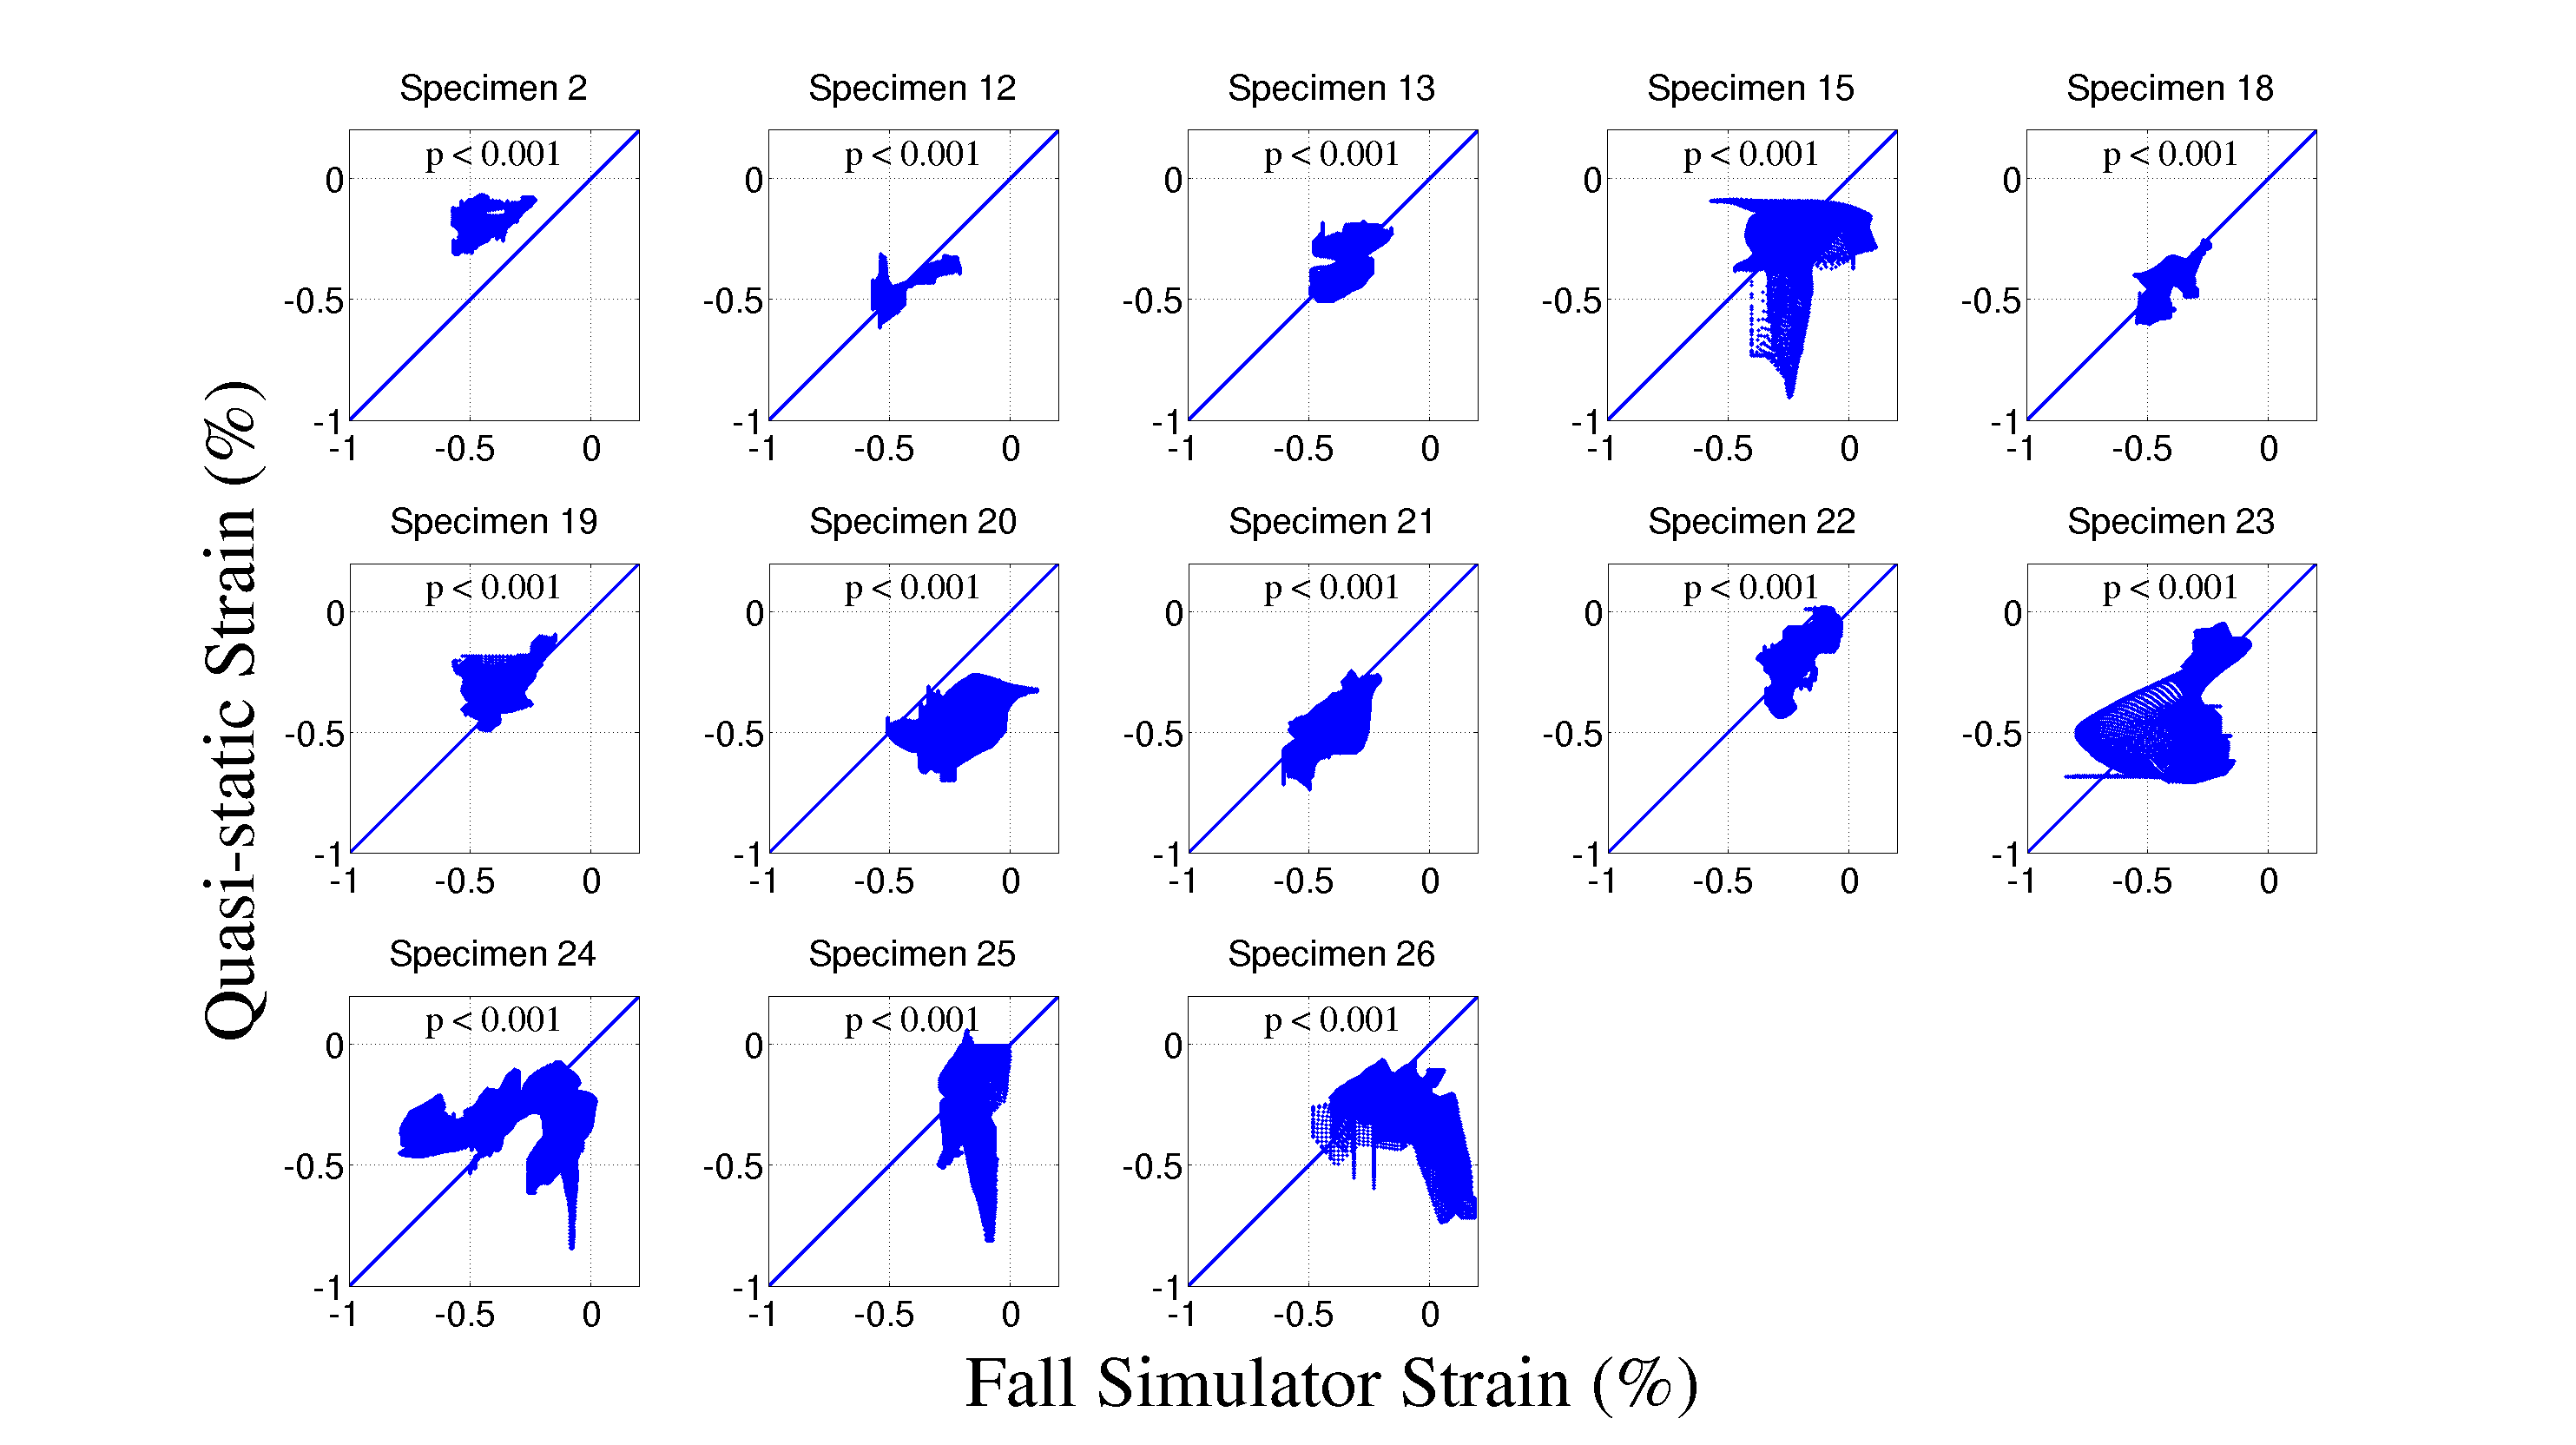
\includegraphics[width=\linewidth]{./fracture/Figures/StrainDiffs}
	\caption[Strain differences for specimens in the simulated group]{\textbf{Strain-strain plots comparing minimum compressive strain between the fall:\ac{QS} and fall:\ac{fs} groups.
	Each point in each plot is at the same location and load, and the \textit{p}-values are the results of a paired t-tests on all points in the point cloud.} Graphic \textcopyright Seth Gilchrist, 2013.}
	\label{fig:StrainDiffs}
\end{figure}
\end{landscape}
} % afterpage

\begin{figure}
	\centering
	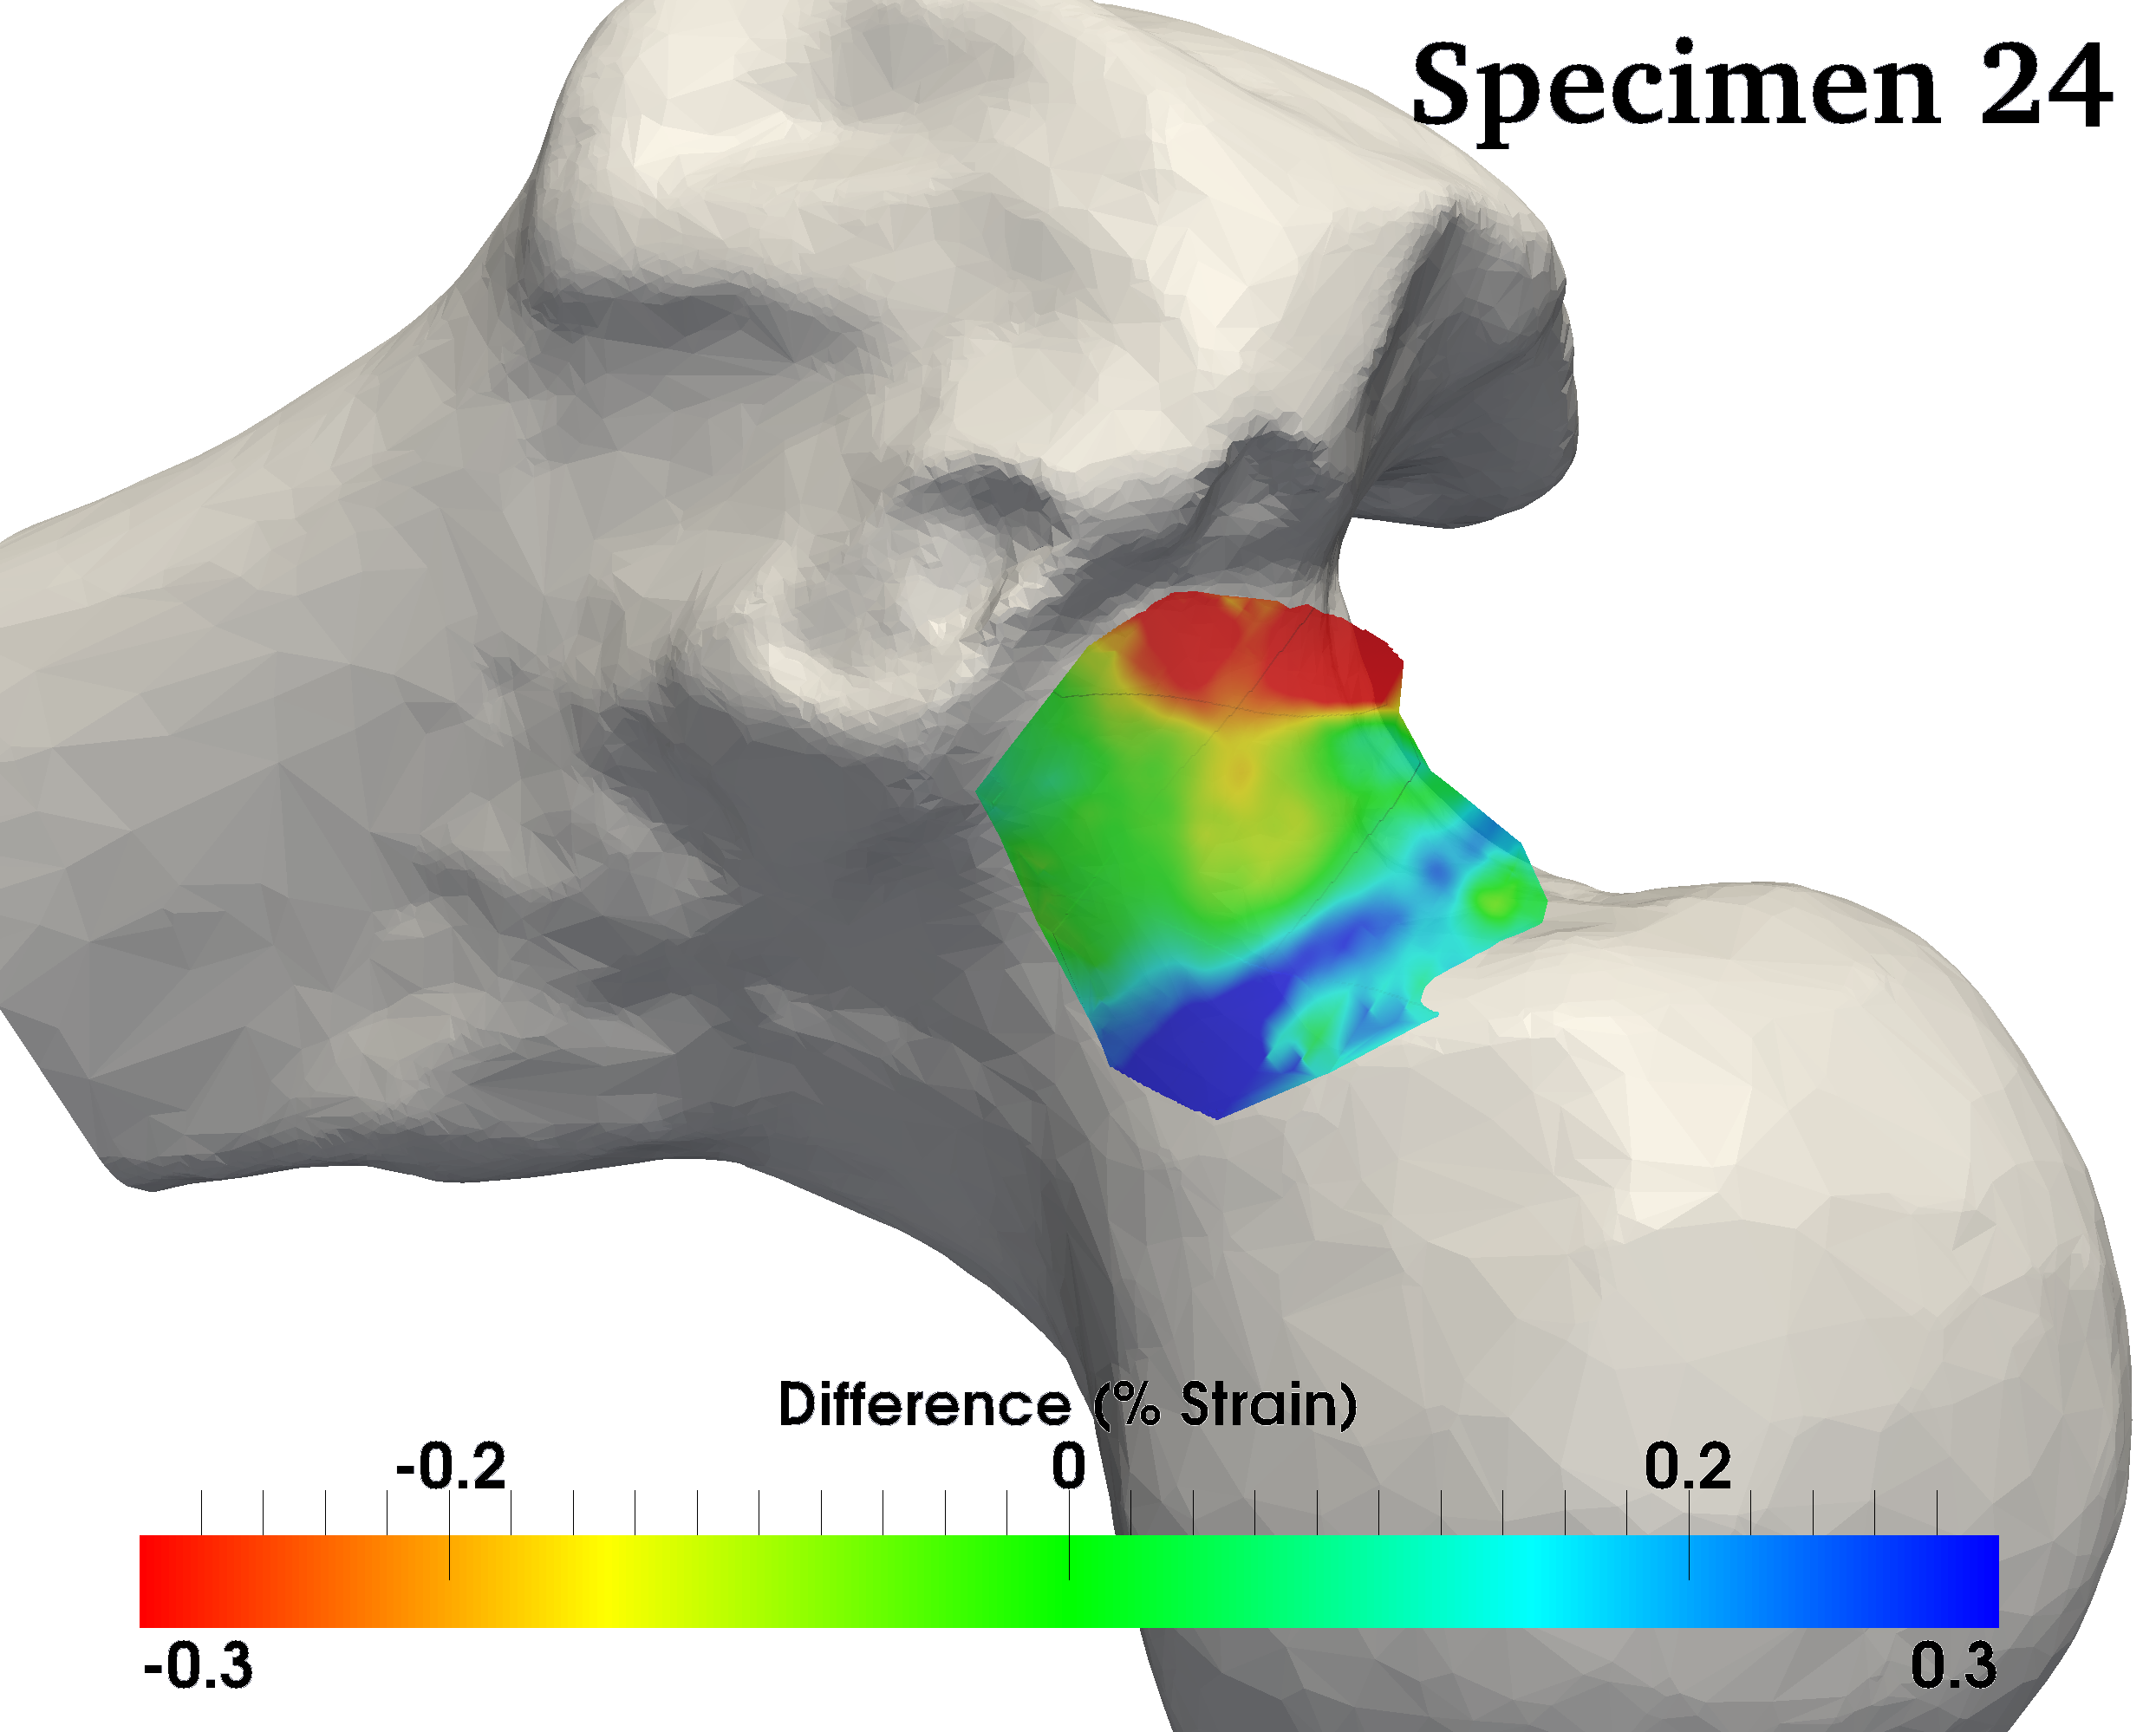
\includegraphics[width=0.9\linewidth]{./fracture/Figures/H1380R_FemurOverlay}
	\caption[Strain differences overlaid on an example bone]{\textbf{Fall:\ac{QS} minus fall:\ac{fs} minimum principal strains at the same load overlaid on the specimen.
	In this case, the fall:\ac{fs} tests had higher strains in the lateral neck and lower strains along the subcapital line.
	The average strain difference for this specimen was 39~\ac{micro-eps}, with a range of [-770, 470]~\ac{micro-eps}.} Graphic \textcopyright Seth Gilchrist, 2013.}
	\label{fig:H1380R_FemurOverlay}
\end{figure}

\begin{table}
	\centering
	\caption{Published fracture locations for laboratory experiments}
	\label{tab:labFx}
	\begin{tabular}{p{8cm} >{\centering}p{2cm} c}
		\toprule
		Author                                  &     Neck     & Trochanteric \\ \midrule
		\citet{backman_proximal_1957}           &      36      &     117      \\
		\citet{lotz_use_1990}                   &      6       &      6       \\
		\citet{weber_proximal_1992}             &      8       &      7       \\
		\citet{courtney_effects_1994} (Elderly) &      5       &      4       \\
		\citet{courtney_effects_1994} (Young)   &      6       &      3       \\
		\citet{pinilla_impact_1996}             &      8       &      3       \\
		\citet{keyak_prediction_2001}           &      4       &      10      \\
		\citet{lochmuller_mechanical_2002}      &      54      &      40      \\
		\textbf{Totals}                         &  \textbf{127} &  \textbf{190} \\ \bottomrule
	\end{tabular} 
\end{table}

\begin{table}
	\centering
	\caption{Published fractures locations for clinical studies}
	\label{tab:clinicalFx}
	\begin{tabular}{p{8cm} >{\centering}p{2cm} c}
		\toprule
		Author                                &      Neck      &  Trochanteric  \\ \midrule
		\citet{michelson_epidemiology_1995}   &       63       &       83       \\
		\citet{lyritis_epidemiology_1996}     &      791       &      995       \\
		\citet{sirois_burden_2009}            &      783       &      1584      \\
		\citet{lefaivre_changes_2011}         &     22313      &     19677      \\			
		\citet{poole_cortical_2012}           &       36       &       39       \\
		\textbf{Totals}                       & \textbf{23986} & \textbf{22378} \\ \bottomrule
	\end{tabular}
\end{table}

Comparison of the fracture outcomes of the current experiments to those published in the clinical literature is complicated by the lack of post fracture x-rays in the current tests.
Clinical fractures are diagnosed and classified using radiological examination, however, in the fall group, the fall simulator often destroyed the greater and lesser trochanter of the specimens post fracture, making radiological examination impossible.
That said, classification as either intra- or extracapsular was possible from fragment analysis and video observation and the current results are in-line with previous tests and clinical observations (Tables~\ref{tab:labFx} and~\ref{tab:clinicalFx}).
The fall:\ac{fs} fractures were split 50/50 between intra- and extracapsular fractures, while the slow group showed a slight tendency toward extracapular fractures.
Both methods gave distributions of fracture types that are representative of what has been observed in the clinical literature.

Examination of the strain values on the surface of the specimens at the same compressive load while being tested with the two protocols showed that average strain over the analysis regions was not statistically different between the two testing protocols, however, no single specimen had the same strain.
These results seem contradictory, however, they are indicative of a random variation in surface strain due to the change in loading protocol.
A cohort of specimens loaded quasi-statically will show, on average, the same strain as those loaded in the impact fall simulator, however, each individual specimen will have a different response in the two tests.
This result has important implications for study design.
If a case-series study is examining the change in strain due to an intervention in which two sufficiently sized cohorts of specimens are treated in two different ways, quasi-static, constant displacement rate simulations will be sufficient to study the effects of the intervention.
However, if a study is examining changes in a specimen specific manner, \ac{eg}, trying to identify the correct intervention to decrease surface strains in a particular specimen, then impact fall simulation is warranted.

It should be noted that alignment errors in the registration process could have led to differences being detected between specimens that were not real.
If the \ac{dic}-measured surfaces were not perfectly aligned, the strain gradients on the surface could manifest as a reconfiguration of strain in the strain-strain plots.
However, each comparison in this study was individually inspected for two features:
\begin{inparaenum}[i\upshape)]
\item \label{item:dic_surf} surface size, extent and off-plane features, and
\item location of strain differences.
\end{inparaenum}
The first item was important for ensuring a reliable registration.
Surfaces that were either flat or described only a portion of a cylindrical surface were eliminated from the comparisons.
Features that were considered sufficient for inclusion of a surface were extension of the surface onto the femoral head or trochanter in a way that provided an out of plane, or off-cylindrical axis registration target.
The second item was a post-processing analysis aimed at identifying if the branches seen in the strain-strain plots were in close physical proximity.
If the locations of strain difference were physically near each other, the surfaces were re-evaluated in terms of (\ref{item:dic_surf}) and either eliminated if the surface was insufficient for accurate alignment, modified if an identifiable feature was driving a misalignment, or accepted if the registration was driven by a sufficiently complex surface.


A few specimens showed redistributions of strain on the anterior superior femoral neck that were, in some cases, quite large.
This reasons for this are unknown, but could be related to failures of cancellous bone below the surface early in the loading which are not visible in the current tests.
Failure within the structure could cause the load path to be altered, which could manifest as a change in pattern and magnitude on the surface.

To our knowledge, this study is the first of its kind to compare the failure locations, and fracture patterns in two populations tested at considerable extremes of loading protocols, as well as to examine the strain fields of individual specimens loaded to sub-failure using different protocols.
Like all \textit{ex-vivo} fracture experiments, this study has some limitations that we did our best to mitigate, but must be considered during interpretation.
First of all, the small number of specimens reduces the power to identify differences between the fall and slow groups.
That said, most of the comparisons between the two methods resulted in statistical results that were sufficiently powerful that more specimens would not have been required.
Once exception to this may be the initial failure location.
It was not seen to be different, but the \textit{p}-value of 0.13 could be considered a trend worth further investigation.
Secondly, the impact testing protocol resulted in the destruction of the specimens and consequently post fracture \ac{a-p} x-rays were not possible.
Since clinical fracture evaluation is carried out using \ac{a-p} x-rays, the results of this work are not directly comparable to clinical outcomes.
However, the classification into intra- and extracapsular fractures should be comparable due to the distinctly different locations of these portions of the proximal femur.
Additionally, some of the fractures were such that they may not have been observed using a-p x-ray examination.
These fractures were hairline fractures along the superior femoral neck, in the coronal plane and may represent failures not yet documented in the clinical literature.
Finally, the strain mapping was carried out only on the superior-anterior surface of the femoral neck, which may not be representative of the proximal femur as a whole.
This fact limits the applicability of the no difference when pooling data result, but it does not limit the applicability of the observations on individual specimens where we can say that in the critical location of the anterior-superior neck, the response is different between the two loading methods.
Additionally, the density of the strain data are much higher than previous tests utilizing strain gauges and thus provides a rich dataset for statistical analysis.

Overall, this work indicates that more biofidelic replication of the fall and fracture scenario may benefit the examination of hip fracture progression.
The changes in final fracture types and the redistribution of strain in some specimens may be indicative of internal mechanics that have heretofore gone unobserved.
The examination of fracture patterns in two similar populations tested in two very different scenarios allowed us to understand how loading mechanism affects failure through rate-dependent failure changes.
Our interpretation of the results lead us to recommend that experiments in which single specimens are treated in different manners with the goal of influencing strain development or fracture behaviour use fall simulation to test outcomes.
However, if general changes in a cohort of specimens are to be observed, quasi-static testing at constant displacement rate, or impact fall simulation can be used.
We believe that future finite element research should concentrate on incorporating strain-rate dependency in material properties, and create specimen-specific models whose fracture predictions are validated using applicable loading rates.
These models could be used to identify the critical load path in a fall to the side, and investigate the effects of changing this load path due to local failures within the cancellous and cortical bone.
This technique could help understand the phenomena of how an initial failure in the trochanter can lead to fracture of the neck in fall simulation.
Ultimately, we aim to understand how forces are transferred in a compromised femur, potentially giving us the tools to develop intervention and screening technologies that would reduce the burden of this devastating condition.
